% Asset ID: AS1TrigonometricRatiosTIKZ-007
% Source: P1-Chp9 pp.31-36
% Related section: Trig Graphs
% Purpose: Sine, cosine and tangent graph sketches
\documentclass[tikz,border=8pt]{standalone}
\usepackage{amsmath}
\usetikzlibrary{angles,quotes,calc,arrows.meta}
\begin{document}
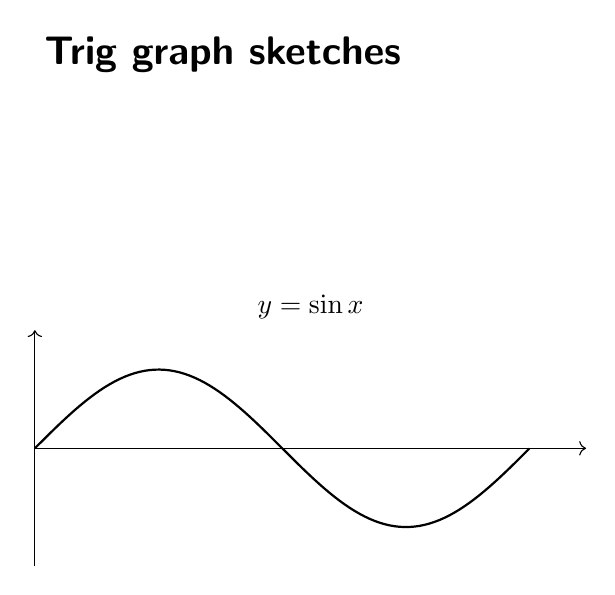
\begin{tikzpicture}[scale=1.0, every node/.style={font=\sffamily}]
\node[font=\sffamily\bfseries\Large, anchor=west] at (0,5) {Trig graph sketches};
\draw[->] (0,0)--(7,0);\draw[->] (0,-1.5)--(0,1.5);\draw[thick,domain=0:6.28,samples=100] plot (\x,{sin(180*\x/3.14159)});\node at (3.5,1.8) {$y=\sin x$};
\end{tikzpicture}
\end{document}
